\section{Long-Term Oceanographic Research with Citizen Scientists}

How do we increase temporal and spatial coverage of the ocean? A single oceanographic research vessel can cover a small fraction of the ocean. During a continuous year at sea, without stopping for fuel or crew change, a single research vessel could cover ∼3\% of ocean-area sampling at a distance of 1 degree, traveling at 10 knots between stations and only stopping at each station for two hours. Despite this being an enormous area, representing 9.7 million km2 (area calculation from the Goode Homolosine projection), it conservatively would cost at least US\$15 million for the boat, the crew, the science, and the scientists. Twenty vessels would be required to operate at this intensity to cover the midlatitude region, putting into perspective the costs of conducting oceanography on a global ocean-basin scale. The carbon footprint of this effort would be enormous. The costs would exceed US\$300 million dollars, and the results would still exclude the entire high-latitude oceans.

Citizen oceanography, specifically science conducted aboard sailing yachts, would overcome many of these hurdles and empower civilian scientists with the pride of data contribution to science, providing an incredible opportunity for outreach as well as improving science education and increasing public awareness. Participation of a small fraction of the thousands of vessels that continuously cruise remote parts of the oceans (Figure 1) could comprise a global oceanographic monitoring network that would boost the predictive power of scientific models. This would be a natural group of citizen scientists inherently motivated by their love of sailing and empirical knowledge of the beauty, power, and vastness of the world's oceans. Given the complexities and importance of the coastal ocean, an obvious question is, why not include coastal recreational sailors in this call to action? The coastal waters present problems related to permitting, and deregulated sampling would infringe on the exclusive economic rights of nations' territorial waters. However, other initiatives such as Ocean Sampling Day [8] can be extended to cover multiple days throughout the year. In partnership with coastal schools and universities, this is a huge pool of citizen scientists and citizen data collectors.

\begin{figure}
\centering
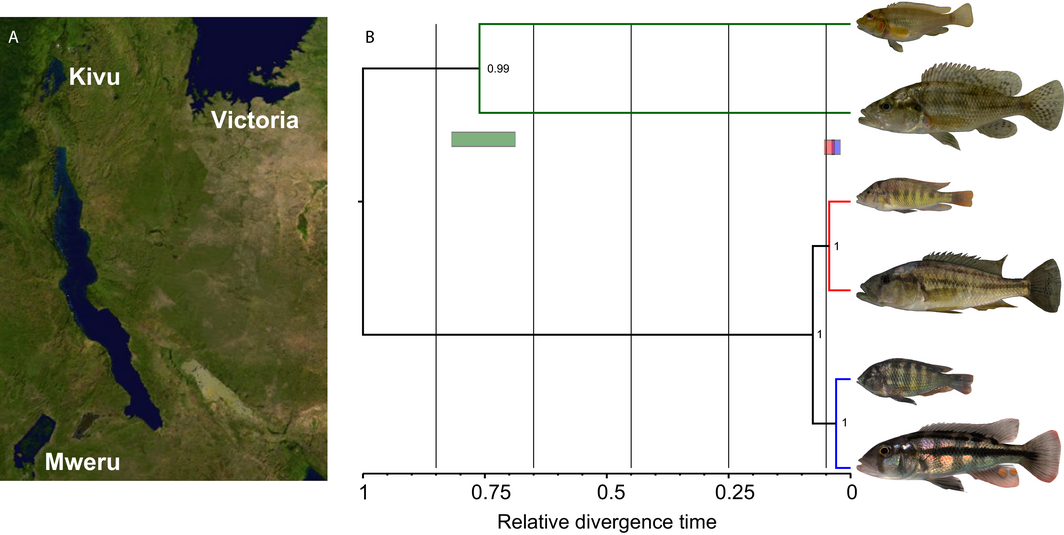
\includegraphics[width=\textwidth]{IndigoV/figures/fig1}
\caption{\textbf{Month-by-month maps of sailing yacht transits around the world.} Data are collected from the YOTREPS network url{http://www.pangolin.co.nz/} of cruising yachts worldwide and plotted with Esri ArcGIS 10.2.1. Density of yacht traffic is highest in red. Note the seasonal patterns of transits in the various oceans: high density of traffic during the “Coconut Milk Run” in the Pacific beginning in April, eastward Atlantic ocean traffic during the boreal summer and westward during the boreal winter, and passages to Alaska in the heart of the boreal summer. Used with permission. Esri, DigitalGlobe, 2014.}
\label{IV_fig1}
\end{figure}

As a specific example, we know relatively little about the inventory of microorganisms and their variability in the oceans. Biological sampling by citizen scientists could be accomplished using mass-produced Niskin bottles, preloaded with fixatives, for flow cytometry and nutrient analysis. A basic conductivity-temperature-depth (CTD) device could be manufactured using standard mass-market consumer electronic practices for measuring physical properties. Inexpensive digital weather stations already exist for recording conditions and are commonplace on small, private vessels. A wide-angle camera and an inexpensive embedded computer could be used to automatically identify and catalogue debris with image-processing software.

Repetitive sampling through time is important to grasp the complexities of dynamic systems (cf. [9]–[11]). The long-term ecological research (LTER) model for understanding ecosystem function and change across relevant temporal scales has produced numerous significant observations [12],[13]. Two important long-term research observatories in the Atlantic (Bermuda Atlantic Time-series Study [BATS]) and Pacific (Hawaiian Ocean Time-series [HOT]) have revolutionized our understanding of biology and chemistry in the ocean [14]. Yet, these are only two stations in the middle of vast oceans.

There is repetitive, seasonal yacht traffic along common sailing routes around the globe (Figure 1). At least 5,000 sailing yachts travel the oceans every year using several popular routes. For example, ∼400 yachts per year embark on the Pacific Coconut Milk Run, which is approximately a 6,000 nautical mile journey from the western US or Panama Canal to New Caledonia in the Southwest Pacific. This popular route is marked by relatively mild weather and easterly trade winds. The Atlantic Ocean has similar seasonal and favorable sailing routes. The trade wind route (westward from Canaries to the Caribbean) is mostly sailed in winter, while the Bermuda-Azores (eastward) is popular in the summer (Figure 1). Both attract hundreds of sailors every year, as they are a part of every sailor's “wish list,” having been used since the Age of Discovery in the early 15th century. If a metadata and sample collection system were in place, sailors on popular routes such as these could be a part of a larger, LTER-like sampling collective. Ocean-going sailors have an extensive network already in place for communication, passage notes, weather, etc. (e.g., \url{http://www.cruiserswiki.org/}; \url{http://pangolin.co.nz/}); expanding this infrastructure is trivial compared to current research vessel costs. These routes can be used to monitor the ocean repetitively for interannual and long-term changes, much like the NWS-COOP or National Phenology Network programs.

Any data gaps in areas with lower density of recreational sailors (e.g., high latitudes) could be filled by engaging commercial shipping companies, which have vessels that operate in those waters [15].

